\documentclass{article}
\usepackage[utf8]{inputenc}
\usepackage[spanish]{babel}
\usepackage{listings}
\usepackage{graphicx}
\graphicspath{ {images/} }
\usepackage{cite}

\begin{document}

\begin{titlepage}
    \begin{center}
        \vspace*{1cm}
            
        \Huge
        \textbf{MULTI-TRIQUI}
            
        \vspace{0.5cm}
        \LARGE
        Proyecto de Informática II
            
        \vspace{1.5cm}
            
        \textbf{Yuribia Arroyave\\
        Fabián Hoyos}
        
    
            
        \vfill
            
        \vspace{0.8cm}
            
        \Large
        Departamento de Ingeniería Electrónica y Telecomunicaciones\\
        Universidad de Antioquia\\
        Medellín\\
        Marzo de 2021
            
    \end{center}
\end{titlepage}

\tableofcontents
\newpage
\section{Introducción}\label{intro}
El triqui es un juego conocino por muchas personas al rededor del mundo, que consiste en un tablero de 9 posiciones (3x3) y dos contrincantes cada uno con una ficha o símbolo diferente, normalmente equis 'X' y ceros '0'; el objetivo principal de cada jugador es lograr poner su símbolo en tres casillas consecutivas, ya sea en horizontal, vertical o diagonal. En cada turno el jugador bvuscará lograr su objetivo, o impedir ser vencido por su contendor.\\\

Este popular juego ha sido el orígen de una gran categoría de juegos informáticos para diferentes plataformas, conocidos como los juegos "tres en raya"\\\

En este proyecto se quiere diseñar un vídeo juego basado en la idea original del "triqui", pero con algunas variantes como veinticuatro casillas en lugar de nueve, con una distribución diferente, y adicionando estrátegias de juego similares a las utilizadas en el ajedrez.

\section{MULTI TRIQUI} \label{Contenido}

El multi triqui es una variación del tradicional triqui de 9 casillas en un cuadro de 3 x 3, donde el objetivo es lograr posicionar el símbolo que representa a un jugador en tres casillas consecutivas; en esta nueva versión se harán modificaciones a este popular juego de "tres en raya" donde cada jugador podrá hacer uno o dos triquis en una jugada y así eliminar fichas de su oponente, como se hace en el ajedrez al capturar fichas del contendor. Así quien logre el mayor número de fichas capturadas de su oponente, reduciendo sus movimientos para que no pueda hacer más triqui, será el ganador de la partida.

\subsection {Tablero}

El tablero estará distribuido en tres cuadrados, uno dentro del anterior, cada cuadrado tendrá en total 8 posiciones: En las esquinas (4) y en los puntos medios de sus lados (4), para un total de veinticuatro (24) posiciones. \\\

Cada posición además de unirse por las líneas demarcadas por los lados de su cuadrado, también se unirá a los otros dos cuadros con líneas entre las esquinas, formando diagonales de tres posiciones; y con líneas entre los puntos medios de los lados, uniendo también tres posiciones (una de cada cuadro).

\subsection {Juego}

Dos participantes, cada uno con doce fichas y turnos intercalados.
En cada turno el participante ubica una de sus fichas en una posición del tablero.\\
A partir del cuarto turno, el participante debe fijarse en ubicar su ficha en un lugar en el que pueda lograr un triqui, o interferir para que su contrincante no lo pueda hacer en su próximo turno.
Si el jugador logra un triqui, puede tomar una ficha de su oponente que esté en el tablero, bajando así sus posibilidades de formar un triqui.\\
Una vez puestas las doce fichas por cada uno de los participantes, el turno será para desplazar alguna de las fichas que tiene en el tablero hasta lograr formar un nuevo triqui, y seguir quitando fichas al oponente.\\
Al retirar fichas del oponente trás realizar triqui, sólo se podrán retirar aquellas fichas que no estén formando ya un triqui. Es decir que las fichas que forman triqui, son fichas aseguradas y no podrán ser capturadas.



\subsection {Desplazamientos}

Las fichas en el tablero se pueden desplazar en horizontal, vertical o diagonal hacia las casillas adyacentes y sólo una casilla por turno. Siempre sobre las líneas demarcadas que unen a las casillas, no se puede hacer saltos de un lado a otro en el cuadro central, es decir de frente o diagonal por el centro del tablero.

\subsection {Triqui}

El triqui se forma en línea recta o diagonal con tres casillas ocupadas por el mismo jugador (su ficha). Al formar un triqui se puede quitar del tablero una ficha del oponente.\\\
Si en un desplazamiento se logra formar dos triquis "Multi triqui", se le quitará al oponente ese mismo número de fichas del tablero, siempre que esas fichas no estén aseguradas por un triqui previo del oponente.\\\
El multi triqui puede estar formado por dos líneas de un cuadro que comparten una misma esquina, o por una diagonal y un lado de un cuadro que comparten una casilla de la diagonal.

\subsection {Fin del juego}

El juego termina una vez uno de los jugadores ya no puede hacer nuevo triqui, ya sea por falta de fichas porque tiene menos de tres o porque sus fichas han sido inmovilizadas, rodeadas por fichas del oponente que le impiden realizar desplazamientos.

\subsection {Diseño}

El juego debe brindar la opción de jugarse por dos personas o de ser jugado por una sola persona con la máquina como oponente.\\
Permitir registrar el nombre de los jugadores.\\
Las fichas a usar en la partida pueden tener diferentes diseños y colores para elegir.\\
El tablero puede brindar difrentes fondos, en particular tener la opción de ser oscuro o claro.\\


\subsubsection{Ilustración Inicial del Juego} \label{imagenes}

En la Figura (\ref{fig:image1}), se presenta una imagen del tablero vacío en un diseño a lápiz sobre cartón.

\begin{figure}[h]
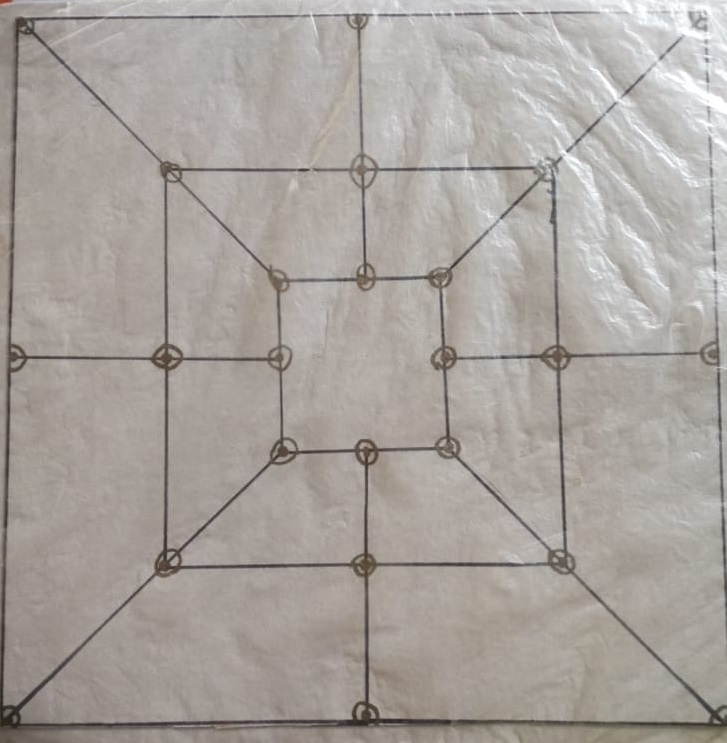
\includegraphics[width=6.25cm]{image1.jpeg}
\centering
\caption{Tablero vacío}
\label{fig:image1}
\end{figure}

En la Figura (\ref{fig:image2}), se presenta una imagen del tablero con fichas.

\begin{figure}[h]
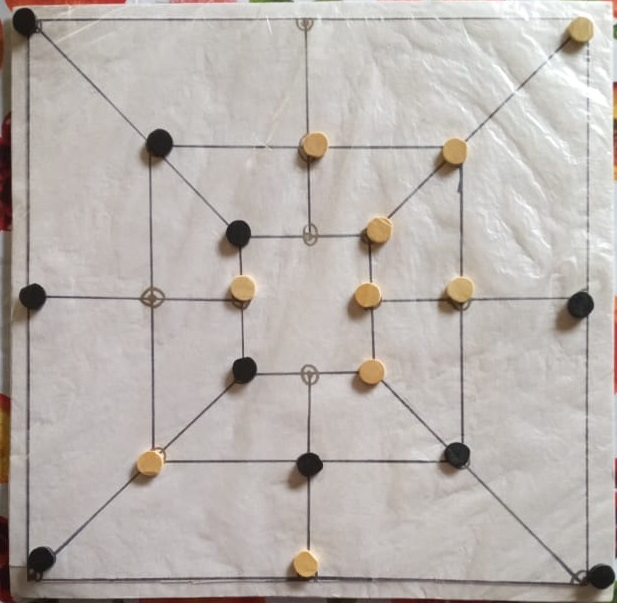
\includegraphics[width=6.25cm]{image2.jpeg}
\centering
\caption{Tablero con fichas}
\label{fig:image2}
\end{figure}

\bibliographystyle{IEEEtran}
\bibliography

\end{document}

Las secciones (\ref{intro}), (\ref{contenido}) y (\ref{imagenes}) dependen del estilo del documento.